\documentclass[a4paper]{article}
\usepackage[pdftex]{hyperref}
\usepackage[latin1]{inputenc}
\usepackage{enumitem}
\usepackage[english]{babel}
\usepackage{a4wide}
\usepackage{amsmath}
\usepackage{array}
\usepackage{amssymb}
\usepackage{algorithmic}
\usepackage{algorithm}
\usepackage{ifthen}
\usepackage{listings}
% move the asterisk at the right position
\lstset{basicstyle=\ttfamily,tabsize=4,literate={*}{${}^*{}$}1}
%\lstset{language=C,basicstyle=\ttfamily}
\usepackage{moreverb}
\usepackage{palatino}
\usepackage{multicol}
\usepackage{tabularx}
\usepackage{comment}
\usepackage{verbatim}
\usepackage{color}

%% pdflatex?
\newif\ifpdf
\ifx\pdfoutput\undefined
\pdffalse % we are not running PDFLaTeX
\else
\pdfoutput=1 % we are running PDFLaTeX
\pdftrue
\fi
\ifpdf
\usepackage[pdftex]{graphicx}
\else
\usepackage{graphicx}
\fi
\ifpdf
\DeclareGraphicsExtensions{.pdf, .jpg}
\else
\DeclareGraphicsExtensions{.eps, .jpg}
\fi

\parindent=0cm
\parskip=0cm

\setlength{\columnseprule}{0.4pt}
\addtolength{\columnsep}{2pt}

\addtolength{\textheight}{5.5cm}
\addtolength{\topmargin}{-26mm}
\pagestyle{empty}

%%
%% Sheet setup
%% 
\newcommand{\coursename}{Secure and Dependable Systems}
\newcommand{\courseno}{CO21-320203}
 
\newcommand{\sheettitle}{Homework}
\newcommand{\mytitle}{}
\newcommand{\mytoday}{\textcolor{blue}{March 28th}, 2019}

% Current Assignment number
\newcounter{assignmentno}
\setcounter{assignmentno}{3}

% Current Problem number, should always start at 1
\newcounter{problemno}
\setcounter{problemno}{1}

%%
%% problem and bonus environment
%%
\newcounter{probcalc}
\newcommand{\problem}[2]{
  \pagebreak[2]
  \setcounter{probcalc}{#2}
  ~\\
  {\large \textbf{Problem \textcolor{blue}{\arabic{assignmentno}}.\textcolor{blue}{\arabic{problemno}}} \hspace{0.2cm}\textit{#1}} \refstepcounter{problemno}\vspace{2pt}\\}

\newcommand{\bonus}[2]{
  \pagebreak[2]
  \setcounter{probcalc}{#2}
  ~\\
  {\large \textbf{Bonus Problem \textcolor{blue}{\arabic{assignmentno}}.\textcolor{blue}{\arabic{problemno}}} \hspace{0.2cm}\textit{#1}} \refstepcounter{problemno}\vspace{2pt}\\}

%% some counters  
\newcommand{\assignment}{\arabic{assignmentno}}

%% solution  
\newcommand{\solution}{\pagebreak[2]{\bf Solution:}\\}

%% Hyperref Setup
\hypersetup{pdftitle={Homework \assignment},
  pdfsubject={\coursename},
  pdfauthor={},
  pdfcreator={},
  pdfkeywords={Secure and Dependable Systems},
  %  pdfpagemode={FullScreen},
  %colorlinks=true,
  %bookmarks=true,
  %hyperindex=true,
  bookmarksopen=false,
  bookmarksnumbered=true,
  breaklinks=true,
  %urlcolor=darkblue
  urlbordercolor={0 0 0.7}
}
% for truth tables
\newcolumntype{C}{>$c<$}

%for new table
\usepackage{multirow}

\begin{document}
\coursename \hfill Course: \courseno\\
Jacobs University Bremen \hfill \mytoday\\
\textcolor{blue}{Dragi Kamov}\hfill
\vspace*{0.3cm}\\
\begin{center}
{\Large \sheettitle{} \textcolor{black}{\assignment}\\}
\end{center}

\problem{}{0}
\solution
\begin{itemize}
    \item[a)]
        \begin{itemize}
        \item[(i)] $ \Theta_L(e) < \Theta_L(f) \implies e \prec f $
        \item[(ii)] $ \Theta_L(e) < \Theta_L(f) \implies f \prec e $
        \end{itemize}
        
        Both of the statements are false, because it is impossible to determine which event happened first according to the clock value. \\
        From the following picture we can see that although $ \Theta_L(e) < \Theta_L(f) $, nothing can be inferred about which event happened first. \\
        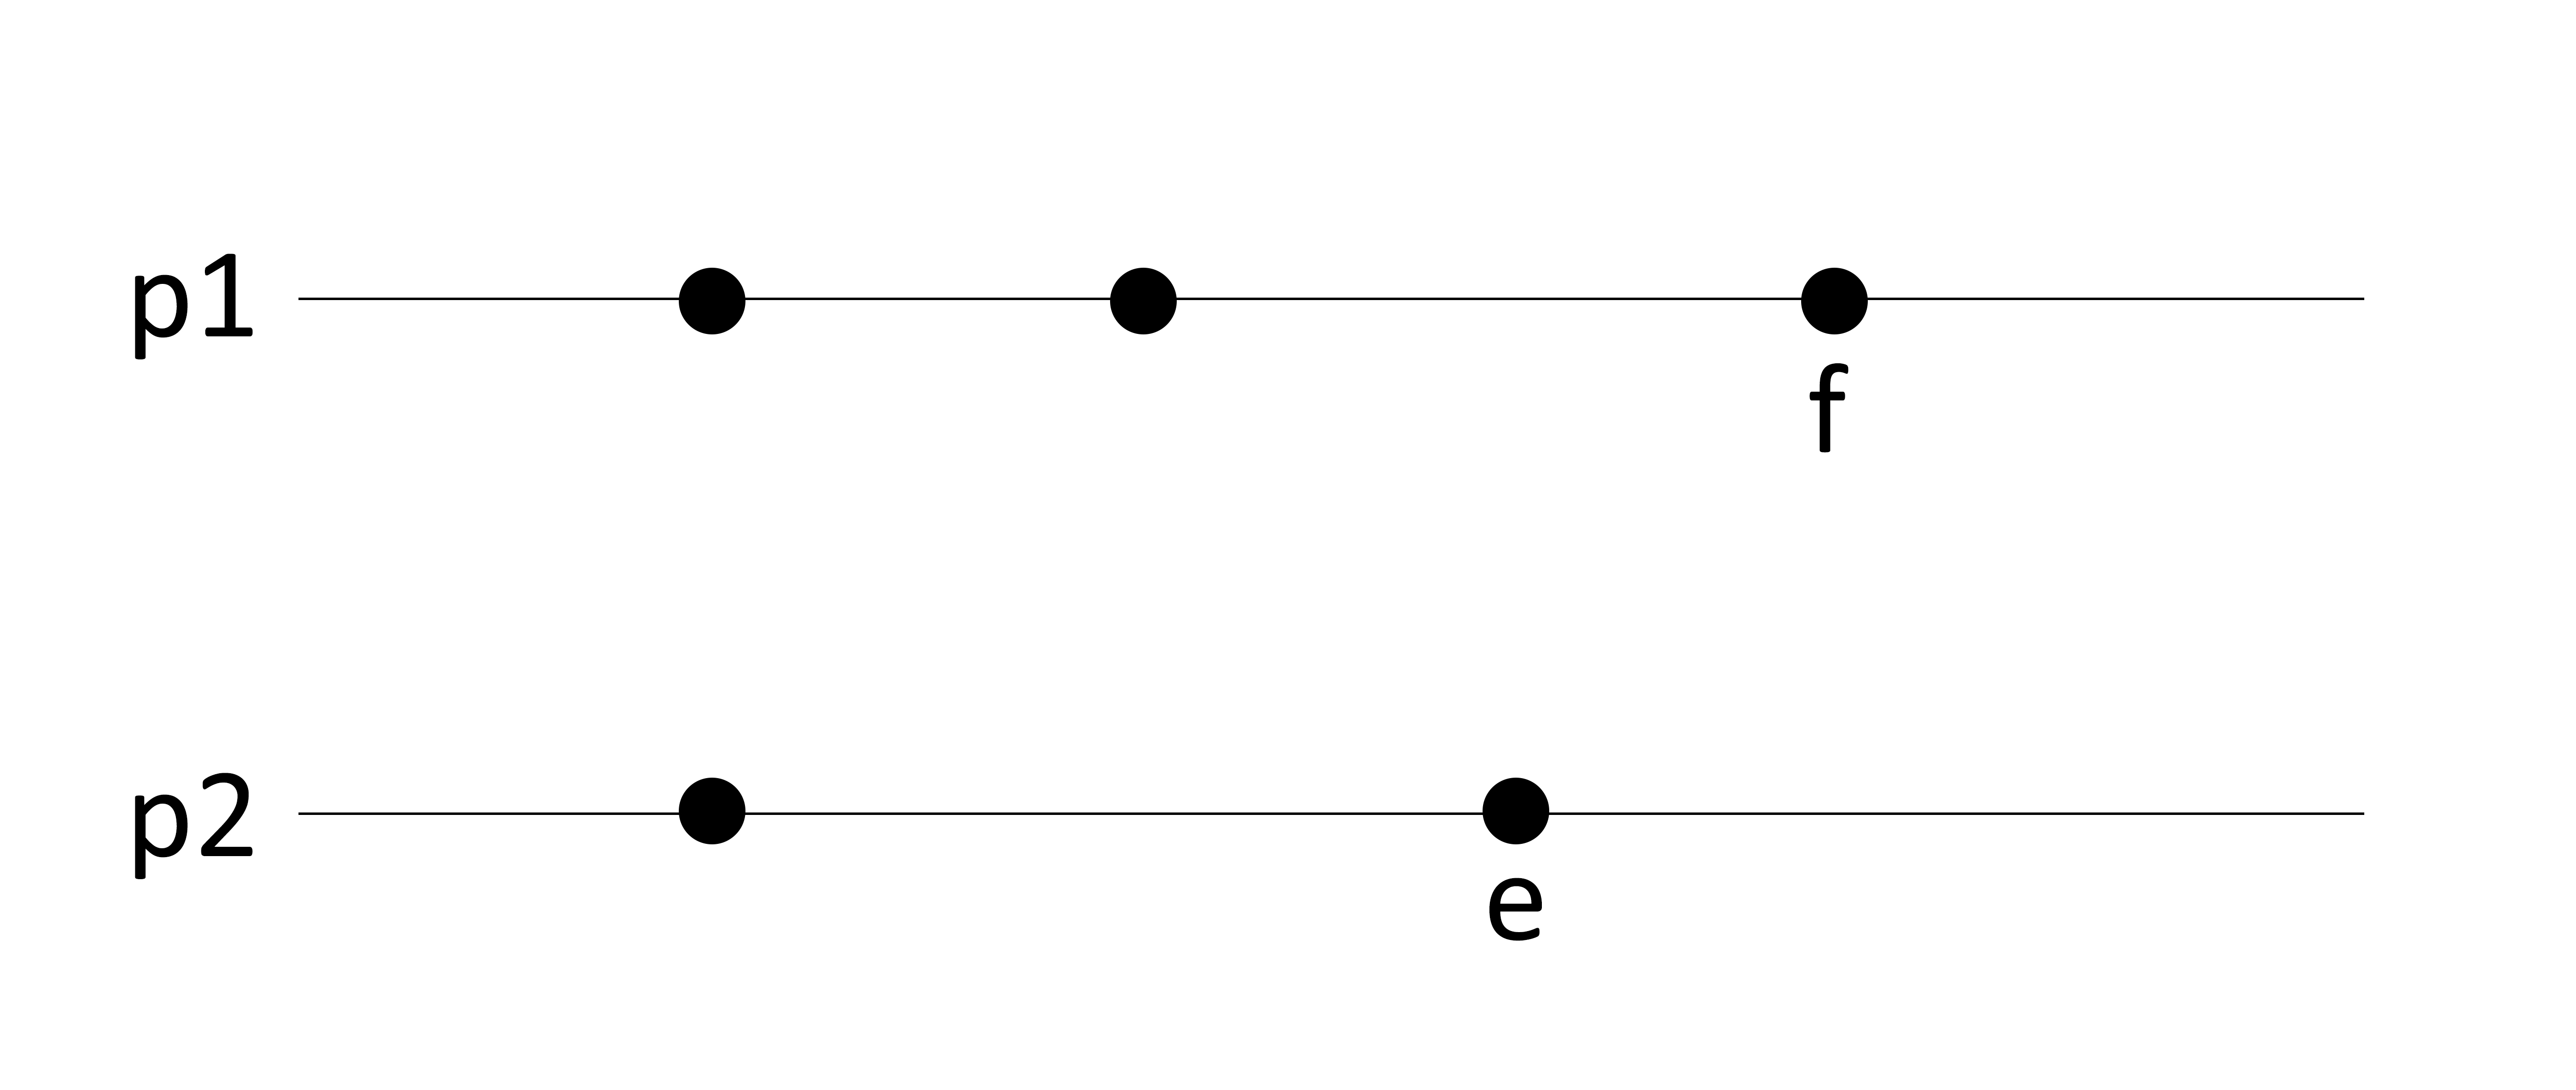
\includegraphics[scale=0.8]{p1.jpg}
    \item[b)]
        \begin{itemize}
        \item[(i)] $ \Theta_V(e) < \Theta_V(f) \implies e \prec f $
        \item[(ii)] $ \Theta_V(e) < \Theta_V(f) \implies f \prec e $
        \end{itemize}
        
        The first statement is true, whereas the second one is false. In order to prove that, I am going to prove the right side of 
        \[e \prec f \iff \Theta_V(e) < \Theta_V(f)\]
        This is equivalent to showing 
        \[!(e \prec f) \rightarrow !(\Theta_V(e) < \Theta_V(f))\]
        Let's suppose $ e $ occurs at $ p_i $ and $ f $ at $ p_j $, and $ e $ doesn't happen before $ b $. Let $ \Theta_V(e)_i = k $. Since $ e $ doesn't happen before $ f $ there is no chain of messages from $ p_i $ to $ p_j $ originating at $ p_i $'s kth step or later and ending at $ p_j $ before $ f $. Thus $ \Theta_V(f)_i < k $. Thus $ !(\Theta_V(e) < \Theta_v(f) $.
    \item[c)] In order to find out whether $ e $ and $ f $ are concurrent we must do an element by element comparison of the corresponding timestamps; if some elements of $ \Theta_V(e) $ are smaller than their $ \Theta_V(f) $ counterparts and some are greater than their matches, then we know that the events are concurrent.
\end{itemize}

\newpage

\problem{}{0}
\solution
\begin{itemize}
    \item[a)] Lamport clock values for all events. \\
    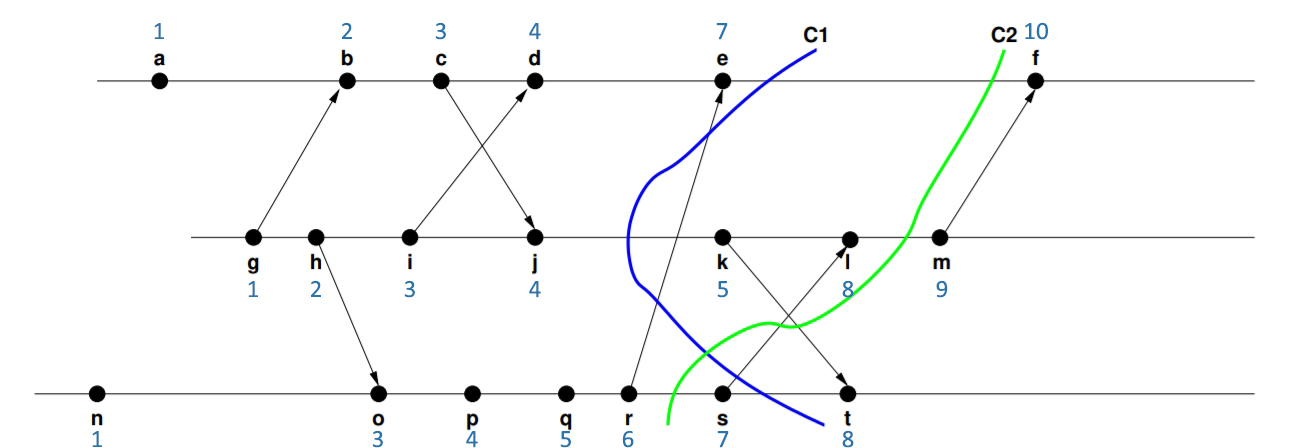
\includegraphics[scale=0.6]{p2.jpg}
    \item[b)] Vector clock values for all events. \\
    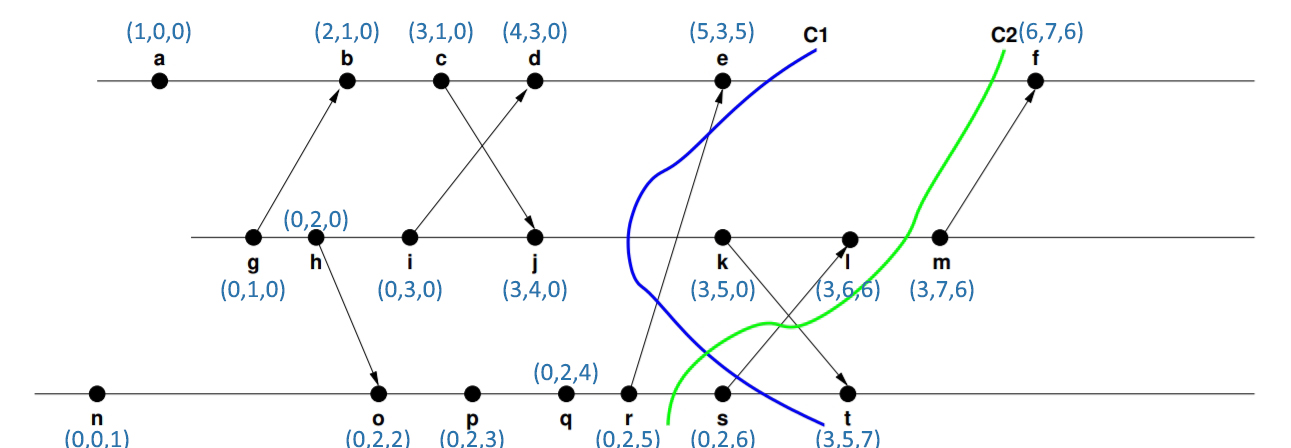
\includegraphics[scale=0.6]{p3.jpg}
    \item[c)] The cut $ C_1 $ is consistent as there is no step outside the cut that happens before steps $ e $, $ j $ and $ s $. On the other hand, cut C2 is not consistent as we can see that $ s $ who happens outside the cut, happens before $ l $ that is inside the cut.
\end{itemize}

\problem{}{0}
\solution
    Referenced from \textcolor{blue}{\href{http://lpd.epfl.ch/site/_media/education/da12-causalbroadcast.ppt}{here}}
    \begin{lstlisting}[escapeinside={(*}{*)}]
    upon event < Init > do 
        for all pi (*$ \in $*) S: VC[pi] := 0; 
        pending := (*$ \varnothing $*)
    
    upon event < rcoBroadcast, m> do
        trigger < rcoDeliver, self, m>; 
        trigger < rbBroadcast, [Data,VC,m]>;
        VC[self] := VC[self] + 1;
    
    upon event <rbDeliver, pj, [Data,VCm,m]> do 
        if pj != self then 
            pending := pending (*$ \cup $*) (pj, [Data,VCm,m]);
            deliver-pending.
    
    procedure deliver-pending is
        While (s, [Data,VCm,m]) (*$ \in $*) pending s.t.
            for all pk: (VC[pk] >=  VCm[pk]) do 
                pending := pending - (s, [Data,VCm,m]);
                trigger < rcoDeliver, self, m>;
                VC[s] := VC[s] + 1.
    \end{lstlisting}
\end{document}
